% Options for packages loaded elsewhere
\PassOptionsToPackage{unicode}{hyperref}
\PassOptionsToPackage{hyphens}{url}
\PassOptionsToPackage{dvipsnames,svgnames,x11names}{xcolor}
%
\documentclass[
  11pt,
  letterpaper,
  DIV=11,
  numbers=noendperiod]{scrartcl}

\usepackage{amsmath,amssymb}
\usepackage{iftex}
\ifPDFTeX
  \usepackage[T1]{fontenc}
  \usepackage[utf8]{inputenc}
  \usepackage{textcomp} % provide euro and other symbols
\else % if luatex or xetex
  \usepackage{unicode-math}
  \defaultfontfeatures{Scale=MatchLowercase}
  \defaultfontfeatures[\rmfamily]{Ligatures=TeX,Scale=1}
\fi
\usepackage{lmodern}
\ifPDFTeX\else  
    % xetex/luatex font selection
    \setmainfont[]{Times New Roman}
\fi
% Use upquote if available, for straight quotes in verbatim environments
\IfFileExists{upquote.sty}{\usepackage{upquote}}{}
\IfFileExists{microtype.sty}{% use microtype if available
  \usepackage[]{microtype}
  \UseMicrotypeSet[protrusion]{basicmath} % disable protrusion for tt fonts
}{}
\makeatletter
\@ifundefined{KOMAClassName}{% if non-KOMA class
  \IfFileExists{parskip.sty}{%
    \usepackage{parskip}
  }{% else
    \setlength{\parindent}{0pt}
    \setlength{\parskip}{6pt plus 2pt minus 1pt}}
}{% if KOMA class
  \KOMAoptions{parskip=half}}
\makeatother
\usepackage{xcolor}
\usepackage[margin=1in]{geometry}
\setlength{\emergencystretch}{3em} % prevent overfull lines
\setcounter{secnumdepth}{5}
% Make \paragraph and \subparagraph free-standing
\makeatletter
\ifx\paragraph\undefined\else
  \let\oldparagraph\paragraph
  \renewcommand{\paragraph}{
    \@ifstar
      \xxxParagraphStar
      \xxxParagraphNoStar
  }
  \newcommand{\xxxParagraphStar}[1]{\oldparagraph*{#1}\mbox{}}
  \newcommand{\xxxParagraphNoStar}[1]{\oldparagraph{#1}\mbox{}}
\fi
\ifx\subparagraph\undefined\else
  \let\oldsubparagraph\subparagraph
  \renewcommand{\subparagraph}{
    \@ifstar
      \xxxSubParagraphStar
      \xxxSubParagraphNoStar
  }
  \newcommand{\xxxSubParagraphStar}[1]{\oldsubparagraph*{#1}\mbox{}}
  \newcommand{\xxxSubParagraphNoStar}[1]{\oldsubparagraph{#1}\mbox{}}
\fi
\makeatother


\providecommand{\tightlist}{%
  \setlength{\itemsep}{0pt}\setlength{\parskip}{0pt}}\usepackage{longtable,booktabs,array}
\usepackage{calc} % for calculating minipage widths
% Correct order of tables after \paragraph or \subparagraph
\usepackage{etoolbox}
\makeatletter
\patchcmd\longtable{\par}{\if@noskipsec\mbox{}\fi\par}{}{}
\makeatother
% Allow footnotes in longtable head/foot
\IfFileExists{footnotehyper.sty}{\usepackage{footnotehyper}}{\usepackage{footnote}}
\makesavenoteenv{longtable}
\usepackage{graphicx}
\makeatletter
\newsavebox\pandoc@box
\newcommand*\pandocbounded[1]{% scales image to fit in text height/width
  \sbox\pandoc@box{#1}%
  \Gscale@div\@tempa{\textheight}{\dimexpr\ht\pandoc@box+\dp\pandoc@box\relax}%
  \Gscale@div\@tempb{\linewidth}{\wd\pandoc@box}%
  \ifdim\@tempb\p@<\@tempa\p@\let\@tempa\@tempb\fi% select the smaller of both
  \ifdim\@tempa\p@<\p@\scalebox{\@tempa}{\usebox\pandoc@box}%
  \else\usebox{\pandoc@box}%
  \fi%
}
% Set default figure placement to htbp
\def\fps@figure{htbp}
\makeatother

\KOMAoption{captions}{tableheading,figureheading}
\makeatletter
\@ifpackageloaded{caption}{}{\usepackage{caption}}
\AtBeginDocument{%
\ifdefined\contentsname
  \renewcommand*\contentsname{Table of contents}
\else
  \newcommand\contentsname{Table of contents}
\fi
\ifdefined\listfigurename
  \renewcommand*\listfigurename{List of Figures}
\else
  \newcommand\listfigurename{List of Figures}
\fi
\ifdefined\listtablename
  \renewcommand*\listtablename{List of Tables}
\else
  \newcommand\listtablename{List of Tables}
\fi
\ifdefined\figurename
  \renewcommand*\figurename{Figure}
\else
  \newcommand\figurename{Figure}
\fi
\ifdefined\tablename
  \renewcommand*\tablename{Table}
\else
  \newcommand\tablename{Table}
\fi
}
\@ifpackageloaded{float}{}{\usepackage{float}}
\floatstyle{ruled}
\@ifundefined{c@chapter}{\newfloat{codelisting}{h}{lop}}{\newfloat{codelisting}{h}{lop}[chapter]}
\floatname{codelisting}{Listing}
\newcommand*\listoflistings{\listof{codelisting}{List of Listings}}
\makeatother
\makeatletter
\makeatother
\makeatletter
\@ifpackageloaded{caption}{}{\usepackage{caption}}
\@ifpackageloaded{subcaption}{}{\usepackage{subcaption}}
\makeatother

\usepackage{bookmark}

\IfFileExists{xurl.sty}{\usepackage{xurl}}{} % add URL line breaks if available
\urlstyle{same} % disable monospaced font for URLs
\hypersetup{
  pdftitle={Bridging the Gap:},
  pdfauthor={Brock Akerman, Hanan Ali, Taylor Cesarski},
  colorlinks=true,
  linkcolor={blue},
  filecolor={Maroon},
  citecolor={Blue},
  urlcolor={Blue},
  pdfcreator={LaTeX via pandoc}}


\title{Bridging the Gap:}
\usepackage{etoolbox}
\makeatletter
\providecommand{\subtitle}[1]{% add subtitle to \maketitle
  \apptocmd{\@title}{\par {\large #1 \par}}{}{}
}
\makeatother
\subtitle{Comparing Employer and Educator Expectations in Small Animal
Dentistry}
\author{Brock Akerman, Hanan Ali, Taylor Cesarski}
\date{2025-06-25}

\begin{document}
\maketitle

\renewcommand*\contentsname{Table of contents}
{
\hypersetup{linkcolor=}
\setcounter{tocdepth}{2}
\tableofcontents
}

\section{Abstract}\label{abstract}

\section{Introduction}\label{introduction}

\subsection{Purpose of project}\label{purpose-of-project}

\subsection{Study details}\label{study-details}

\section{Data}\label{data}

\subsection{Data Description}\label{data-description}

Two separate surveys were administered to mutually exclusive groups:
veterinary employers who have worked with students, and educators who
have taught those students. There was no overlap between these
groups---no evidence suggests that any surveyed student was both taught
by an educator and later employed by a participating employer.

The employer dataset consists of responses from 29 participants, while
the educator dataset includes 43 participants. This difference in
response count suggests greater willingness among educators to engage
with the survey.

Additionally, survey completion time differed between groups. Educators,
on average, spent more time completing the survey than employers. While
the survey did not ask participants to explain their response time, this
difference may reflect greater engagement or the tendency for more
elaborated responses among educators. A box plot below illustrates the
distribution of survey duration (in minutes) by group.

\begin{center}
\pandocbounded{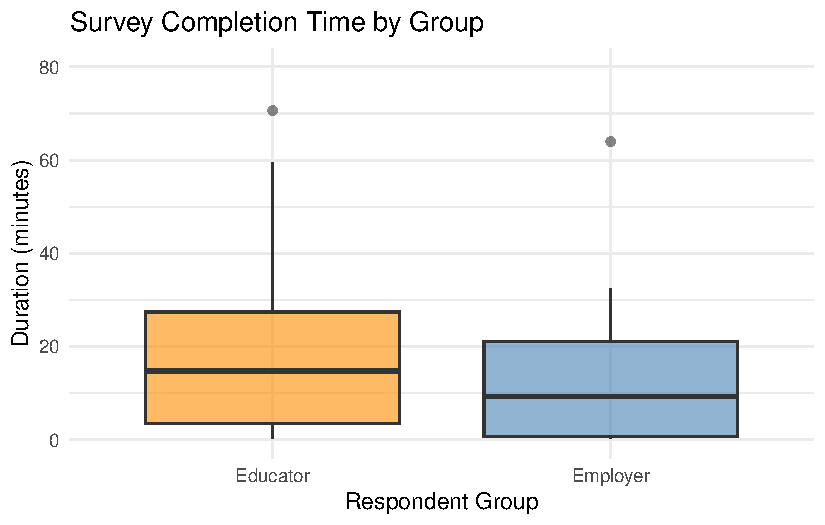
\includegraphics[keepaspectratio]{Final-Project_files/figure-pdf/Data_Desc_01-1.pdf}}
\end{center}

Regarding the proportion of the survey completed, employer responses
were more variable---spanning the full range from partial to full
completion. In contrast, educators tended to complete more of the
survey, with a concentration near full completion and a less pronounced
left tail. The density plot below visualizes these differences in survey
progress across groups.

\begin{center}
\pandocbounded{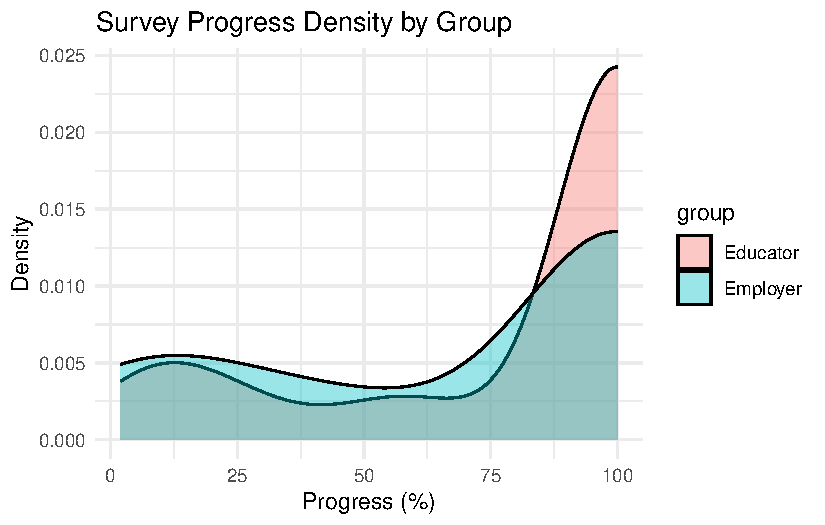
\includegraphics[keepaspectratio]{Final-Project_files/figure-pdf/Data_Desc_02-1.pdf}}
\end{center}

From the educators dataset we could talk about: * Q27; How long have you
been teaching DVM students in the clinical training portion of a DVM
program? * Q28; Does your institution have a teaching hospital? * Q29;
On average, how many dental procedures does your primary care service
perform each week?

From the employers dataset we could talk about: * Q33; Which of the
following best describes your job setting or organization? * Q36; On
average, how many dental procedures does your
practice/oganization/institution perform each week * Q37; Which of the
following best describes the person who completed this survey?

\subsection{Data Source}\label{data-source}

Survey data were collected using Qualtrics, a cloud-based experience
management platform commonly used for gathering feedback and sentiment
across workforce domains. Participants were recruited via email
invitation sent by the researcher, using pre-existing contact lists.
Participation was voluntary and anonymized.

\subsection{Preprocessing Description}\label{preprocessing-description}

Although the employer and educator datasets shared a similar structure,
they were not identical. Most preprocessing steps were applied uniformly
across both datasets, with minor deviations where needed.

The datasets were imported into the RStudio environment (version
2024.04.1 Build 748). A new variable was created to label the data
source (``Educator'' or ``Employer'') for later grouping and
visualization. The existing respondent\_id column served as a unique
identifier and was treated as the primary key.

Initial cleaning involved removing extraneous metadata included by
Qualtrics---such as survey start and end times, IP addresses,
geolocation data, and question display logic---all of which were
irrelevant to the analysis. These columns were trimmed to streamline the
dataset for subsequent transformation and statistical work.

Column names in the original Qualtrics export were alphanumeric but
often ambiguous and misleading. Many variable names did not match the
corresponding survey question numbers. Our team manually mapped the
exported column names to their corresponding survey questions and
responses by referencing adjacent metadata fields and using deductive
reasoning. This process allowed us to build an index-based column naming
structure, which greatly improved the manageability and interpretability
of the dataset.

Before diving into question-specific analysis, we first identified the
subset of survey questions relevant to our research objectives. All
unrelated or out-of-scope items were removed. This step reduced the
employer dataset from 176 columns to 100, and the educator dataset from
171 columns to 102.

Several formatting inconsistencies also needed to be resolved. Some
multi-select questions appeared in the form of comma-separated text
responses within a single column, while others were exported into
multiple binary columns. Additionally, for certain questions, a response
option that received zero selections was dropped entirely by Qualtrics.
To standardize these issues, we implemented a script to ``explode''
comma-separated responses into individual binary columns. For dropped
columns, we manually reintroduced them as zero-filled dummy variables to
preserve the full response structure.

Finally, we filtered out participants who answered less than half of the
survey. We also excluded:

\begin{itemize}
\item
  Employers who responded ``No'' to the question: ``Do you work with
  early career veterinarians (someone who has graduated from a DVM
  program after May 2021)?''
\item
  Educators who responded ``No'' to: ``Do you teach in any capacity of
  the dental curriculum at your institution?''
\end{itemize}

After all preprocessing steps, the final cleaned datasets consisted of
13 employer participants and 30 educator participants.

\section{Statistical Methods}\label{statistical-methods}

\subsection{Research Question
Answered}\label{research-question-answered}

\subsection{Method Description}\label{method-description}

\section{Results}\label{results}

\subsection{Findings}\label{findings}

\subsection{Statistical Analysis}\label{statistical-analysis}

\section{Discussion/Conclusion}\label{discussionconclusion}

\subsection{Interpretation of Results}\label{interpretation-of-results}

\subsection{Implications of the Study}\label{implications-of-the-study}

\subsection{Limitations}\label{limitations}

\subsection{Recommendations}\label{recommendations}

\subsection{Summary of Key Findings}\label{summary-of-key-findings}

\subsection{Final Thoughts}\label{final-thoughts}

\section{Appendix}\label{appendix}




\end{document}
